%%%%%%%%%%%%%%%%%%%%%%%%%%%%%%%%%%%%%%%%%
% Wenneker Assignment
% LaTeX Template
% Version 2.0 (12/1/2019)
%
% This template originates from:
% http://www.LaTeXTemplates.com
%
% Authors:
% Vel (vel@LaTeXTemplates.com)
% Frits Wenneker
%
% License:
% CC BY-NC-SA 3.0 (http://creativecommons.org/licenses/by-nc-sa/3.0/)
% 
%%%%%%%%%%%%%%%%%%%%%%%%%%%%%%%%%%%%%%%%%

%----------------------------------------------------------------------------------------
%	PACKAGES AND OTHER DOCUMENT CONFIGURATIONS
%----------------------------------------------------------------------------------------

\documentclass[11pt]{scrartcl} % Font size

%%%%%%%%%%%%%%%%%%%%%%%%%%%%%%%%%%%%%%%%%
% Wenneker Assignment
% Structure Specification File
% Version 2.0 (12/1/2019)
%
% This template originates from:
% http://www.LaTeXTemplates.com
%
% Authors:
% Vel (vel@LaTeXTemplates.com)
% Frits Wenneker
%
% License:
% CC BY-NC-SA 3.0 (http://creativecommons.org/licenses/by-nc-sa/3.0/)
% 
%%%%%%%%%%%%%%%%%%%%%%%%%%%%%%%%%%%%%%%%%

%----------------------------------------------------------------------------------------
%	PACKAGES AND OTHER DOCUMENT CONFIGURATIONS
%----------------------------------------------------------------------------------------

\usepackage{amsmath, amsfonts, amsthm} % Math packages

\usepackage{listings} % Code listings, with syntax highlighting

\usepackage[english]{babel} % English language hyphenation

\usepackage{graphicx} % Required for inserting images
\graphicspath{{Figures/}{./}} % Specifies where to look for included images (trailing slash required)

\usepackage{booktabs} % Required for better horizontal rules in tables

\numberwithin{equation}{section} % Number equations within sections (i.e. 1.1, 1.2, 2.1, 2.2 instead of 1, 2, 3, 4)
\numberwithin{figure}{section} % Number figures within sections (i.e. 1.1, 1.2, 2.1, 2.2 instead of 1, 2, 3, 4)
\numberwithin{table}{section} % Number tables within sections (i.e. 1.1, 1.2, 2.1, 2.2 instead of 1, 2, 3, 4)

\setlength\parindent{0pt} % Removes all indentation from paragraphs

\usepackage{enumitem} % Required for list customisation
\setlist{noitemsep} % No spacing between list items

%----------------------------------------------------------------------------------------
%	DOCUMENT MARGINS
%----------------------------------------------------------------------------------------

\usepackage{geometry} % Required for adjusting page dimensions and margins

\geometry{
	paper=a4paper, % Paper size, change to letterpaper for US letter size
	top=2cm, % Top margin
	bottom=2cm, % Bottom margin
	left=2cm, % Left margin
	right=2cm, % Right margin
	headheight=0.75cm, % Header height
	footskip=1.5cm, % Space from the bottom margin to the baseline of the footer
	headsep=0.75cm, % Space from the top margin to the baseline of the header
	%showframe, % Uncomment to show how the type block is set on the page
}

%----------------------------------------------------------------------------------------
%	FONTS
%----------------------------------------------------------------------------------------

\usepackage[utf8]{inputenc} % Required for inputting international characters
\usepackage[T1]{fontenc} % Use 8-bit encoding

\usepackage{fourier} % Use the Adobe Utopia font for the document

%----------------------------------------------------------------------------------------
%	SECTION TITLES
%----------------------------------------------------------------------------------------

\usepackage{sectsty} % Allows customising section commands

\sectionfont{\vspace{6pt}\centering\normalfont\scshape} % \section{} styling
\subsectionfont{\normalfont\bfseries} % \subsection{} styling
\subsubsectionfont{\normalfont\itshape} % \subsubsection{} styling
\paragraphfont{\normalfont\scshape} % \paragraph{} styling

%----------------------------------------------------------------------------------------
%	HEADERS AND FOOTERS
%----------------------------------------------------------------------------------------

\usepackage{scrlayer-scrpage} % Required for customising headers and footers

\ohead*{} % Right header
\ihead*{} % Left header
\chead*{} % Centre header

\ofoot*{} % Right footer
\ifoot*{} % Left footer
\cfoot*{\pagemark} % Centre footer
 % Include the file specifying the document structure and custom commands

%----------------------------------------------------------------------------------------
%	TITLE SECTION
%----------------------------------------------------------------------------------------
\usepackage{float}
\title{	
	Homework 1
}
\usepackage{xcolor}
\lstset{
    columns=fixed,       
    numbers=left,                                        % 在左侧显示行号
    frame=none,                                          % 不显示背景边框
    backgroundcolor=\color[RGB]{245,245,244},            % 设定背景颜色
    keywordstyle=\color[RGB]{40,40,255},                 % 设定关键字颜色
    numberstyle=\footnotesize\color{darkgray},           % 设定行号格式
    commentstyle=\it\color[RGB]{0,96,96},                % 设置代码注释的格式
    stringstyle=\rmfamily\slshape\color[RGB]{128,0,0},   % 设置字符串格式
    showstringspaces=false,                              % 不显示字符串中的空格
    language=c++,                                        % 设置语言
}
\author{Yuan Jiahao 2019010070} % Your name

\date{\normalsize\today} % Today's date (\today) or a custom date

\begin{document}

\maketitle % Print the title

%----------------------------------------------------------------------------------------
%	FIGURE EXAMPLE
%----------------------------------------------------------------------------------------

\section{Todo}
Run the given serial code of general matrix-matrix multiplication (GEMM). Try to
exchange the order of the loops, try to add OpenMP directive \textit{\#pragma omp parallel for} to
different loops to parallelize them, verify the correctness of the results, test performance, and
write them in the report;
\section{Hardware Environment of the Machine }
The machine's CPU is Intel Core I7-8700,3.2GHz with 6 cores and 12 threads.And the memory is 32GB,DDR4,3200MHz.And the system is windows subsystem for linux,Ubuntu 20.04.
\section{Results}
Before my results,I have some statements to declare.The most important thing is that no matter how weird the experimental data is,I ensure they are true and have been measured at least 3 times.\label{abcc}
\subsection{the original serial code}
	\subsubsection{experimental result}
		\begin{figure}[H]
			\centering
			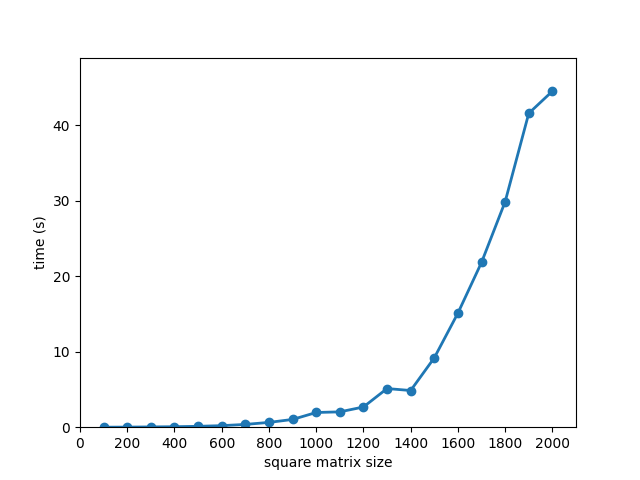
\includegraphics[width=0.8\textwidth]{reftime.png}
			\caption{running time of the original serial code}
			\label{}
		\end{figure}
		\begin{figure}[H]
			\centering
			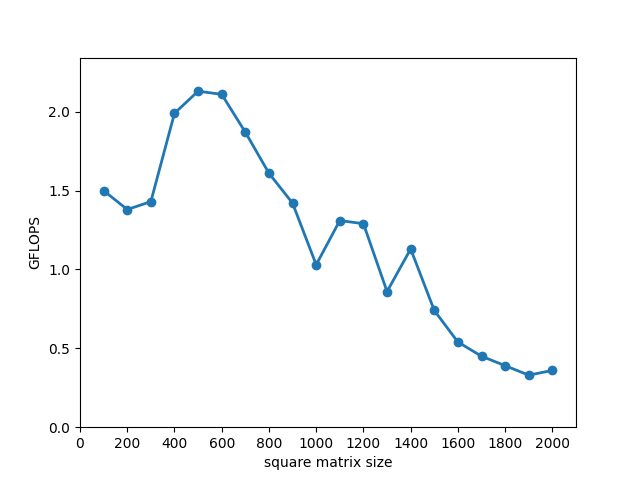
\includegraphics[width=0.8\textwidth]{refgflops.png}
			\caption{floating-point operation performance of the original serial code}
			\label{daf}
		\end{figure}
	\subsubsection{Analysis}
	As the size of matrix grows, the running time of the serial code grows exponentially,which can be correspondingly found in the figure \ref{daf},where the floating-point operation performance drops quickly.

	Meanwhile,another interesting thing can be found only in figure \ref{daf} is that the floating-point operation performance keeps rising and reaches its peak at the size of matrix being 600.

	A conjecture is that the CPU cache helps the performance of the serial code,and when the size of matrix is larger than 600,the cache miss rate raise, finally causing the performance drop.
\subsection{serial codes with the order of the loops exchanged}
	To help have a better insight of the exchanging of loops's impact,I put them in the same graph as below.The different sequence of the same three letter means the sequence of the for loops.
	\subsubsection{experimental result}
		\begin{figure}[H]
			\centering
			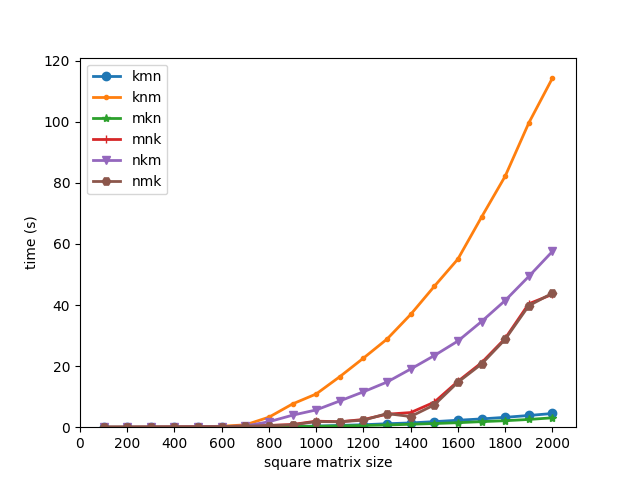
\includegraphics[width=0.8\textwidth]{6time.png}
			\caption{running time of the serial code with the order of the loops exchanged}
			\label{sb1}
		\end{figure}
		\begin{figure}[H]
			\centering
			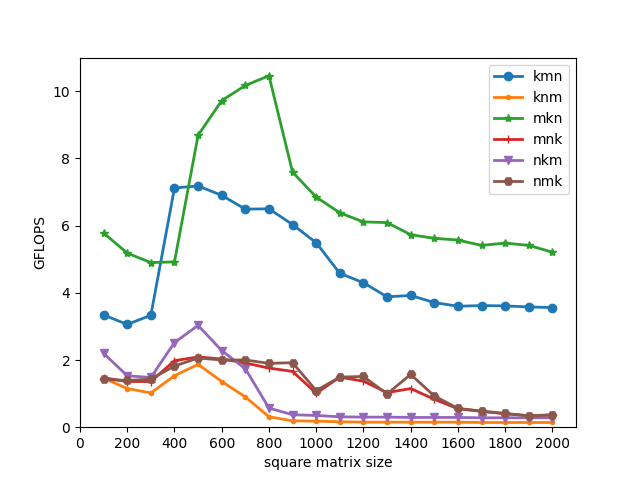
\includegraphics[width=0.8\textwidth]{6gflops.png}
			\caption{floating-point operation performance of the serial code with the order of the loops exchanged}
			\label{sb2}
		\end{figure}
		\subsubsection{Analysis}
		Just as the statement in \ref{abcc},although the graph looks a bit weird since the performance of six groups is supposed to be symmetrical,but obviously wether  figure \ref{sb1} or figure \ref{sb2} is somewhat abnormal and I don't know why.

		The original serial code sequence is ``mnk''.On a macro level, both graphs can be divided into three groups. The performance of each group should be similar. We found that with the increase of the matrix size, except for the ``mkn'' and ``kmn'' group, the calculation time of other groups increased,so is the decline of floating-point calculation performance.And the performance of  ``knm'' and ``nkm'' group drops much slowly than the other, almost reaches to a liner line at last.Anyway, they peaked in the range of matrix sizes from 400 to 800, which corresponds to what we concluded in the previous subsection.Another interesting point is that as long as we put the n loop in the innermost layer, we will get a better result, and a very gentle performance degradation.

		A conjecture is that when n for loop is in the innermost layer,the array C will be loaded after than array A and B,causing writing and reading C both in cache,thus improving the performance.


\subsection{the parallel code of adding OpenMP instruction statements on different for loops}\label{adfa}
	I only measured the original serial code with OpenMP instruction statements on different for loops,and here is the result.
	\subsubsection{experimental result}
		\begin{figure}[H]
			\centering
			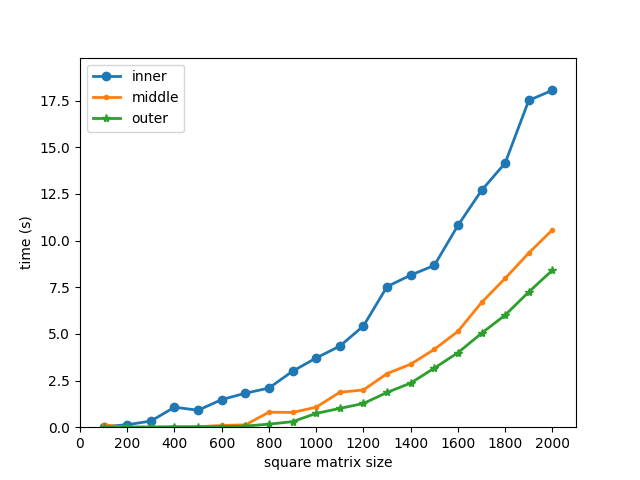
\includegraphics[width=0.8\textwidth]{3time.png}
			\caption{running time of the parallel code}
			\label{}
		\end{figure}
		\begin{figure}[H]
			\centering
			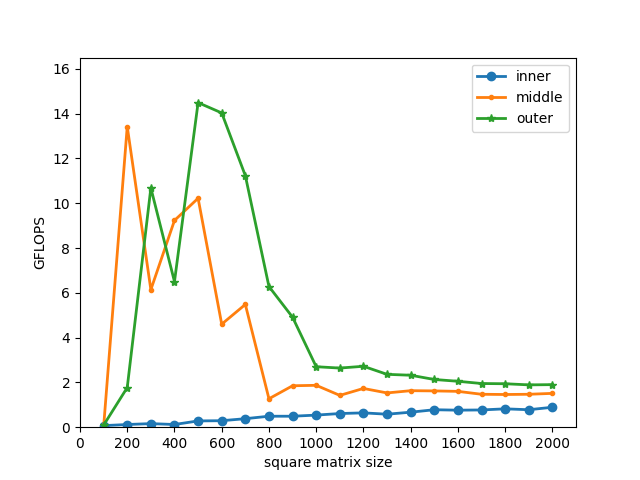
\includegraphics[width=0.8\textwidth]{3gflops.png}
			\caption{floating-point operation performance of the parallel code}
			\label{}
		\end{figure}
	\subsubsection{Analysis}
	No matter which set of data it is, it rises in the early stage, peaks when the matrix size is around 600, and then becomes a horizontal line after the matrix size reaches 1000.

First of all, let's look at the final result. No matter where the instructions are added, it can maintain the level of 1 GFLOPS, which is much better than the 0.5 GFLOPS of the original serial version.And the parallel version of the algorithm does not degrade as the size of the matrix increases, and stabilizes at O(n).

Then it is compared between the three. It can be found that the more parallel instructions are applied to the outer layer, the better the performance. This should be because of the performance loss of starting a new process. If parallel instructions are loaded into the loop, it will cause the C language to create and destroy processes frequently.
\subsection{the parallel code of OpenBLAS}
	\subsubsection{experimental result}
		\begin{figure}[H]
			\centering
			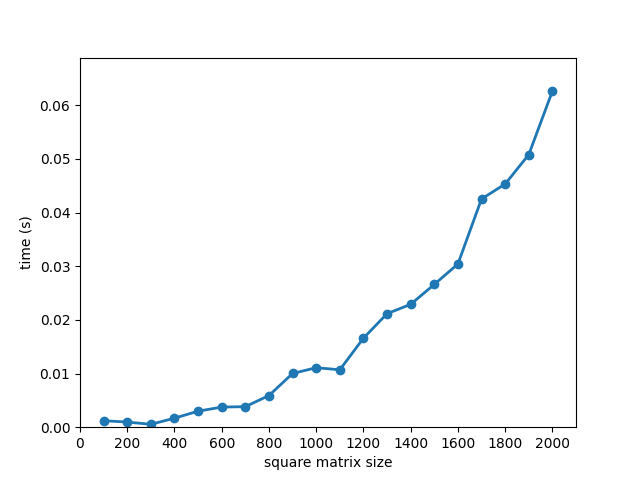
\includegraphics[width=0.8\textwidth]{openblastime.png}
			\caption{running time of the parallel code of OpenBLAS}
			\label{}
		\end{figure}
		\begin{figure}[H]
			\centering
			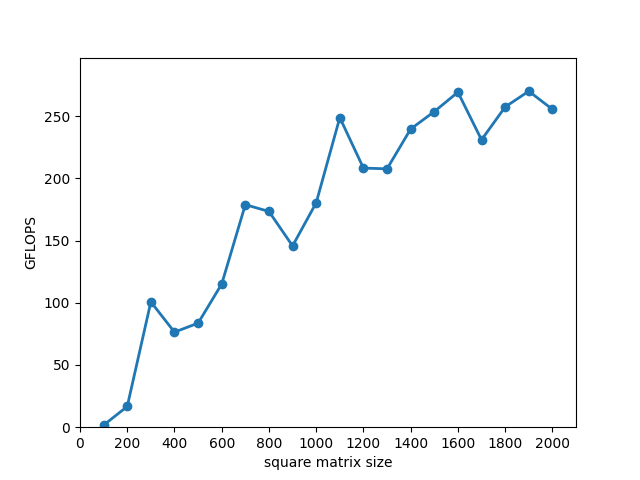
\includegraphics[width=0.8\textwidth]{openblasgflops.png}
			\caption{floating-point operation performance of the parallel code of OpenBLAS}
			\label{}
		\end{figure}
		\subsubsection{Analysis}
		Incredible! The performance of openBLAS is simply beyond my imagination. Not only does its performance not decrease as the size of the matrix increases, but it gets higher and higher. In addition, the performance of the openBLAS version is also more than 40 times the best of all the algorithms previously tested.

I am very curious about how openBLAS has done the magic optimization to get such an excellent performance.
\subsection{Original GEMM code optimized}
	\subsubsection{thinking of optimization}
		So,how can we optimize a GEMM code?Inspired by the chapter \ref{adfa},I'm going to split the big GEMM problem into small parts by the equation shown below:
\begin{figure}[H]
	\centering
	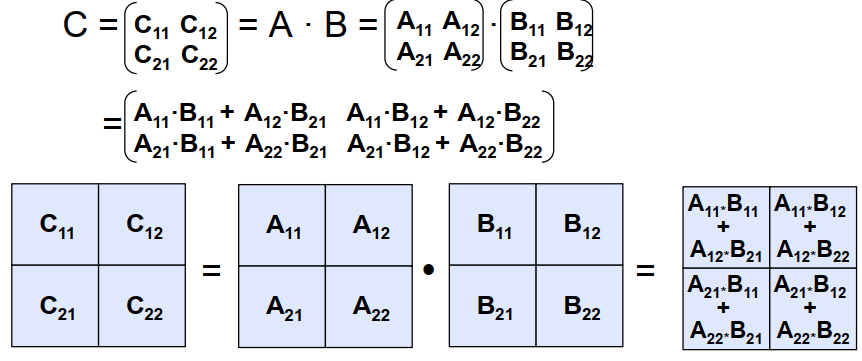
\includegraphics[width=0.8\textwidth]{eq.png}
	\caption{matrix multiplication split equation}
	\label{}
\end{figure}
And the split will end at the matrix size of 800 where the program performance is the best,which makes the best use of cache.After which,I'm going to apply Strassen's Matrix Multiply to reduce the actual number of calculation.

However,somehow the optimization ended at the first step,which is attached at the end of the homework,might due to the wrong memory allocate or access.Due to the limited time,I dropped it and tried somewhat different strategies.

I picked the second step and tried to apply Strassen's Matrix Multiply to the origin given ref code,which not only reduces the number of calculation,but also reduces the number of loop,since control is not free.

Here is the contrast:
\begin{figure}[H]
	\centering
	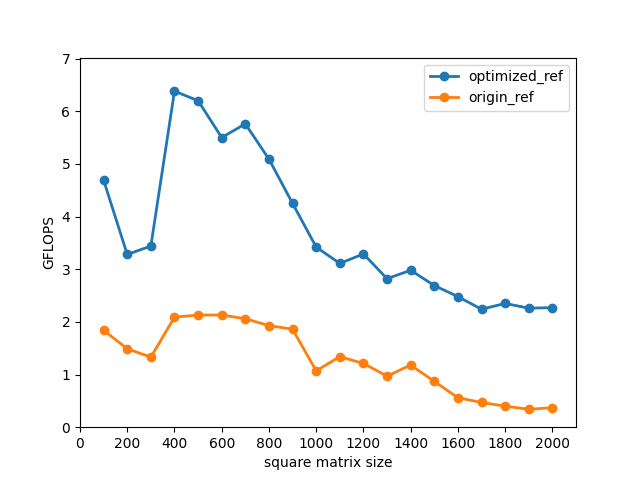
\includegraphics[width=0.8\textwidth]{sb.png}
	\caption{optimized contrast with original}
	\label{}
\end{figure}
See,the optimization works,but performance still drops with the size of the matrix grow.
\newpage
\section{Appendix}
	\begin{lstlisting}[language=c++]
double *mul(double *A, double *B, int m, int k, int n)
{
  double *C = (double *)malloc(sizeof(double) * m * n);
  for (int mi = 0; mi < m; mi++)
  {
    for (int ni = 0; ni < n; ni++)
    {
      for (int ki = 0; ki < k; ki++)
        C[mi * n + ni] += A[mi * k + ki] * B[ki * n + ni];
    }
  }
  return C;
}

double *optm(double *A, double *B, int len)
{
  if (len < 800)
  {
    return mul(A, B, len, len, len);
  }
  int newSize = len * len / 4;
  double *a1 = (double *)malloc(sizeof(double) * newSize);
  double *a2 = (double *)malloc(sizeof(double) * newSize);
  double *a3 = (double *)malloc(sizeof(double) * newSize);
  double *a4 = (double *)malloc(sizeof(double) * newSize);
  double *b1 = (double *)malloc(sizeof(double) * newSize);
  double *b2 = (double *)malloc(sizeof(double) * newSize);
  double *b3 = (double *)malloc(sizeof(double) * newSize);
  double *b4 = (double *)malloc(sizeof(double) * newSize);
  for (int i = 0; i < len / 2; i++)
  {

    int offset = i * len / 2 * sizeof(double);
    memcpy(a1 + offset, A + i * len, len / 2 - 1);
    memcpy(a2 + offset, A + i * len + len / 2, len / 2-1);
    memcpy(a3 + offset, A + len / 2 * len + i * len, len / 2-1);
    memcpy(a4 + offset, A + len / 2 * len + i * len + len / 2, len / 2-1);
    memcpy(b1 + offset, B + i * len, len / 2-1);
    memcpy(b2 + offset, B + i * len + len / 2, len / 2-1);
    memcpy(b3 + offset, B + len / 2 * len + i * len, len / 2-1);
    memcpy(b4 + offset, B + len / 2 * len + i * len + len / 2, en / 2-1);
  }

  double *c1a = optm(a1, b1, len / 2);
  double *c1b = optm(a2, b3, len / 2);
  double *c2a = optm(a1, b2, len / 2);
  double *c2b = optm(a2, b4, len / 2);
  double *c3a = optm(a3, b1, len / 2);
  double *c3b = optm(a4, b3, len / 2);
  double *c4a = optm(a3, b2, len / 2);
  double *c4b = optm(a4, b4, len / 2);
  for (int i = 0; i < newSize; i++)
  {
    c1a[i] += c1b[i];
    c2a[i] += c2b[i];
    c3a[i] += c3b[i];
    c4a[i] += c4b[i];
  }
  double *c = (double *)malloc(sizeof(double) * len * len);
  memcpy(c, c1a, newSize);
  memcpy(c + newSize, c2a, newSize);
  memcpy(c + newSize * 2, c3a, newSize);
  memcpy(c + newSize * 3, c4a, newSize);
  return c;
}
	\end{lstlisting}


\end{document}
